\documentclass{article}
\usepackage{graphicx}

\begin{document}
\title{Classification of activities on Netgear router}
\author{Abhinav Narain}
\maketitle

\section{Mirai Activity and Results}
\subsection{Benchmarks}
We want some micro benchmarks to suggest how good or bad the technique
we are using.


As suggested by Kyle, I have simulated malware activity, instead of
running actual malware mirai. Last report mentioned that it would be
difficult to detect idle activity of the malware. As expected, we
cannot distinguish every instruction execution using EMI.

\begin{itemize}
\item DNS packet flood attack
\item UDP packets with payload of 1460 bytes
\item UDP packets with payload of 730 bytes
\item Router with default firmware running (Idle)
\item Computating
\end{itemize}

There are set of benchmarks I wanted to do but was unable to proceed
and reasons that it was not possible.
\begin{itemize}
\item Experiments with measurements of L1, L2, L3 caches
  \begin{itemize}
  \item Router does not have many levels of caches as dmesg shows~\ref{subsec:dmesg}
  \end{itemize}
\item copying a file (using Linux command \textit{dd})
  \begin{itemize}
  \item Does not have enough memory to copy files for recording it
  \end{itemize}
\end{itemize}

Figure~\ref{fig:setup} shows the testbed setup on the wireless network.


\subsection{Expected Output of EMI}
\begin{figure}[h]
\centering
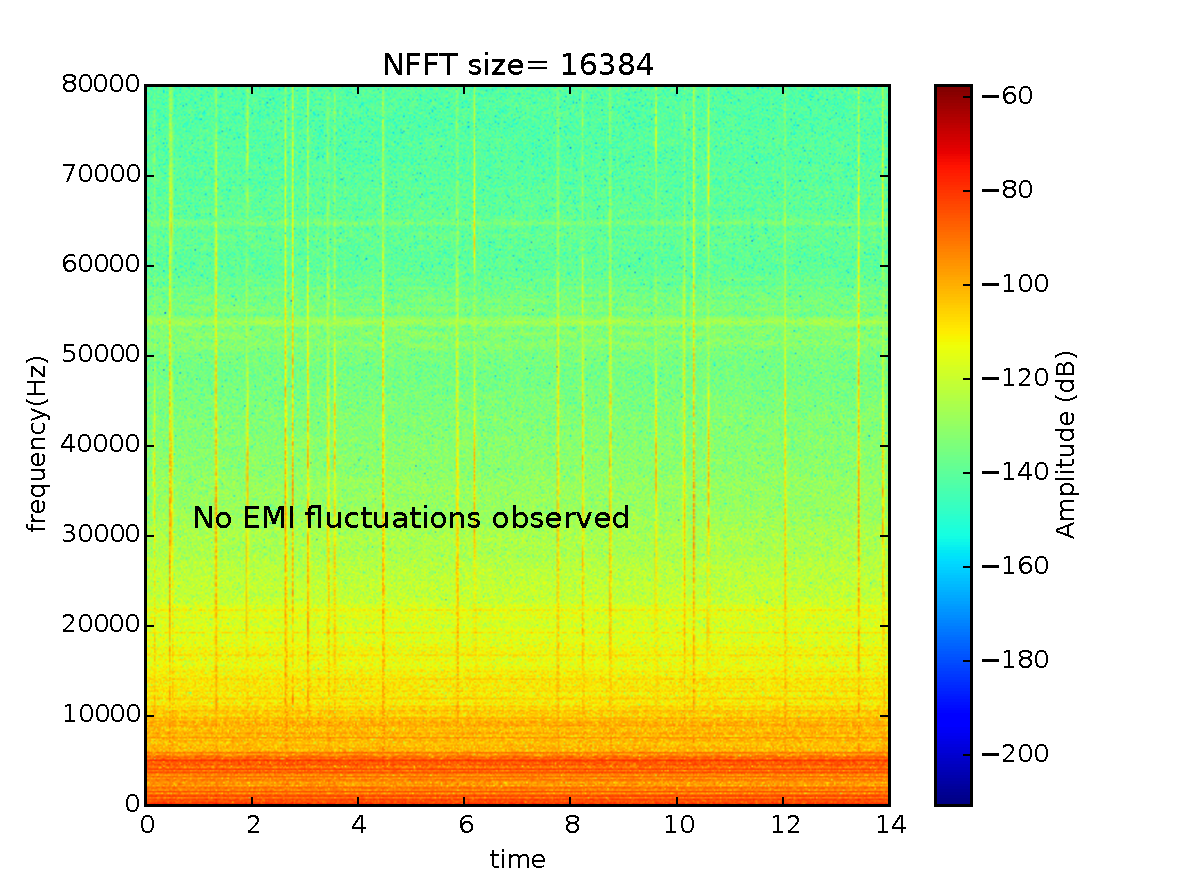
\includegraphics[width=\textwidth]{exec_2_m_16384.pdf}
\caption{Mirai noise profile on Raspberry Pi. Sampling rate$=1e6$, $N=2^{14}$, Resolution (fs/N)=61.035 Hz}
\label{fig:raspi_mirai}
\end{figure}

\section{Comments}
\begin{enumerate}
\item The results are dependent on the hardware. Raspberry Pi did not
  show any activity using our hardware, while the Netgear Router shows
  significant EMI variation  
\item EMI is not very effective in detecting stealthy malware. A
  malware can \textit{sleep} for random time period (for example in
  \textit{mirai} to evade signature detection.  
\item This is not an end all solution and can or cannot work, highly
  depending on the hardware.
\item I have also pursued finding if we could use some bulbs etc. to
  do a distributed attack from bunch of IoT devices together.
  
\end{enumerate}
\subsection{dmesg output}\label{subsec:dmesg}
\begin{lstlisting}
Cached:             6284 kB
[    0.000000] Primary instruction cache 64kB, VIPT, 4-way, linesize 32 bytes.
[    0.000000] Primary data cache 32kB, 4-way, VIPT, cache aliases, linesize 32 bytes
[    0.000000] Dentry cache hash table entries: 16384 (order: 4, 65536 bytes)
[    0.000000] Inode-cache hash table entries: 8192 (order: 3, 32768 bytes)
[    0.086171] Mount-cache hash table entries: 1024 (order: 0, 4096 bytes)
[    0.093221] Mountpoint-cache hash table entries: 1024 (order: 0, 4096 bytes)
\end{lstlisting}






\end{document}




